%\documentclass[dvipdfmx,a4paper,12pt]{amsart}
\documentclass[dvipdfmx,a4paper,11pt]{report} %titleとe-mailをコメントアウトする．


%%% Packages %%%
\setlength{\lineskip}{0pt}

% --- 和文フォント設定 (ゴシックを使うなら) ---amsartを使う時はコメントアウト
\renewcommand{\kanjifamilydefault}{\gtdefault}
\usepackage{otf}          % min10を避けるため
\usepackage{pxrubrica}    % 和文ルビ

% --- 基本パッケージ ---
\usepackage{graphicx}
\usepackage[all]{xy}
\usepackage{wrapfig}
\usepackage{pgfplots}
\usepackage{color}
\usepackage[dvipsnames]{xcolor}

% --- 数学関連 ---
\usepackage{amsmath,amssymb,amsthm,amsfonts,mathtools}
\usepackage{amscd,dsfont,bigdelim,braket,physics,mathrsfs,bm}

% --- 書式・リスト関連 ---
\usepackage{latexsym}
\usepackage{setspace}
\usepackage{multirow}
\usepackage{enumerate}
\usepackage{enumitem}

% --- コメント・取消線など ---
\usepackage{comment}
\usepackage[normalem]{ulem} % \emph の下線化を抑止（cancelと共存）

% --- URL・文字コード ---
\usepackage{url}
% \usepackage[utf8]{inputenc}  % ← 使用しているエンジンがuplatexなら不要、pdflatexなら有効に

% --- showkeys（常に表示） ---
%\usepackage{showkeys}
%\renewcommand*{\showkeyslabelformat}[1]{%
 %\fbox{\parbox{1.6cm}{\normalfont\tiny\sffamily#1\vspace{6mm}}}%
%}
% --- hyperrefは最後に読み込む ---
\usepackage[dvipdfmx,colorlinks,linkcolor=blue,anchorcolor=blue,citecolor=blue]{hyperref}

%%% レイアウト調整 %%%
%%% レイアウト調整（geometryに統一） %%%
\usepackage[
  top=30mm,        % 上余白
  bottom=30mm,     % 下余白
  left=25mm,       % 左余白
  right=25mm,      % 右余白
  headheight=12pt, % ヘッダー高さ（必要なら）
  headsep=10mm,    % ヘッダーと本文の間
  footskip=32pt,   % 本文とフッターの距離
  includehead,     % ヘッダー分も高さに含める
  includefoot      % フッター分も高さに含める
]{geometry}

%%% 行間調整（適宜 1.2 などに変更） %%%
\usepackage{setspace}
\setstretch{1.1}

% --- 段落設定 --- 文字の行間ならここを変更する
\setlength{\parskip}{5pt}   % 段落間のスペース
\setlength{\parindent}{0pt}   % 段落先頭の字下げをなくす


%%% 追加（重複なし）パッケージ・設定 %%%

% --- 目次の体裁調整 ---
%\usepackage{tocloft}
%\renewcommand{\contentsname}{目次} % 日本語化
%\setlength{\cftbeforesecskip}{0pt}
%\setlength{\cftbeforesubsecskip}{0pt}
%\setlength{\cftbeforesubsubsecskip}{0pt}

% --- セクション見出しの体裁調整 ---
%\usepackage{titlesec}
%\titleformat*{\section}{\Large\bfseries}
%\titleformat*{\subsection}{\large\bfseries}
%\titlespacing*{\section}{0pt}{1.5ex plus .2ex minus .2ex}{0.8ex plus .1ex}
%\titlespacing*{\subsection}{0pt}{1.0ex plus .2ex minus .2ex}{0.5ex plus .1ex}

% --- ヘッダー／フッター設定 ---
%\usepackage{fancyhdr}
%\pagestyle{fancy}
%\fancyhf{}
%\rhead{岩井 雅崇}
%\lhead{大阪大学 数学専攻}
%\cfoot{\thepage}


% -- enumerate, itemize行間設定
\usepackage{enumitem} % デフォルト設定
\setlist[itemize]{itemsep=3pt, parsep=0pt}
\setlist[enumerate]{itemsep=3pt, parsep=0pt}
% "変更する際は右を使う" \setlength{\parskip}{0cm} % 段落間\setlength{\itemsep}{5pt} % 項目間

% --- tcolorbox 設定 ---%\begin{tcolorbox}[mybox]と使う
\usepackage[most]{tcolorbox}
\tcbuselibrary{breakable, skins, theorems}
\tcbset{
  mybox/.style={
    colback = white,
    colframe = green!35!black,
    fonttitle = \bfseries,
    breakable = true
  }
}

% --- TikZ 設定 ---
\usepackage{tikz}
\usetikzlibrary{positioning, arrows.meta, fit, calc, backgrounds}
\pgfdeclarelayer{background}
\pgfdeclarelayer{foreground}
\pgfsetlayers{background,main,foreground}

% --- footnote がページをまたがない設定 ---
\interfootnotelinepenalty=10000

% --- 目次に表示する階層の深さ ---
\setcounter{tocdepth}{2}

% --- 日本語目次---
\usepackage{pxjahyper}

%--newtheorem%--newcommand----

\newtheorem{thm}{Theorem}[section] 
\newtheorem{theo}[thm]{Theorem}
\newtheorem{cor}[thm]{Corollary}
\newtheorem{prop}[thm]{Proposition}
\newtheorem{conj}[thm]{Conjecture}
\newtheorem*{mainthm}{Theorem}
\newtheorem{deflem}[thm]{Definition-Lemma}
\newtheorem{lem}[thm]{Lemma}
\theoremstyle{definition} 
\newtheorem{defn}[thm]{Definition}
\newtheorem{propdefn}[thm]{Proposition-Definition} 
\newtheorem{lemdefn}[thm]{Lemma-Definition} 
\newtheorem{thmdefn}[thm]{Theorem-Definition} 
\newtheorem{eg}[thm]{Example} 
\newtheorem{ex}[thm]{Example} 
\newtheorem{ques}[thm]{Question}
\newtheorem{remin}[thm]{Reminder}
\theoremstyle{remark}
\newtheorem{rem}[thm]{Remark}
\newtheorem{setup}[thm]{Setup}
\newtheorem{obs}[thm]{Observation}
\newtheorem{notation}[thm]{Notation}
\newtheorem{cl}{Claim}
\newtheorem{claim}[thm]{Claim}
\newtheorem{assup}[thm]{Assumption}
\newtheorem{step}{Step}
\newtheorem*{clproof}{Proof of Claim}
\newtheorem{cln}[thm]{Claim}
\newtheorem*{ack}{Acknowledgements} 
\numberwithin{equation}{section}
\newtheorem{case}{Case}

\newcommand{\rk}[0]{\operatorname{rk}}
\newcommand{\supp}[0]{\operatorname{Supp}}
\newcommand{\Rad}[0]{\operatorname{Rad}}
\newcommand{\Sha}[0]{\operatorname{Sha}}
\newcommand{\sha}[0]{\operatorname{sha}}
\newcommand{\eend}[0]{\operatorname{End}}
\newcommand{\codim}[0]{\operatorname{codim}}
\newcommand{\nd}[0]{\operatorname{nd}}
\renewcommand{\rank}[0]{\operatorname{rank}}
\newcommand{\degree}[0]{\operatorname{deg}}
\newcommand{\Exc}[0]{\operatorname{Exc}}
\newcommand{\pr}{{\rm pr}}
\newcommand{\id}{{\rm id}}
\newcommand{\Sym}{{\rm Sym}}
\newcommand{\End}[0]{\operatorname{End}}
\newcommand{\Coker}[0]{\operatorname{Coker}}

\newcommand{\Supp}{{\rm Supp}}
\newcommand{\Hom}[0]{\mathscr{H}\!\textit{om}}
\newcommand{\Ext}[0]{\mathscr{E}\!\textit{xt}}
\newcommand{\GL}[0]{\operatorname{GL}}
\newcommand{\SheafHom[1]}{\mathscr{H}\!\!\!\text{\calligra om}_{\,{#1}}}
\newcommand{\PGL}[0]{\mathbb{P}\GL(r,\C)}

\newcommand{\Alb}{{\rm Alb}}
\newcommand{\verti}{{\rm vert}}
\newcommand{\hor}{{\rm hor}}
\newcommand{\univ}{{\rm univ}}
\newcommand{\Tor}{{\rm tor}}
\newcommand{\shaf}{\mathrm{sha}}
\newcommand{\Shaf}{\mathrm{Sha}}
\newcommand{\reg}{{\rm{reg}}}
\newcommand{\sing}{{\rm{sing}}}
\newcommand{\qt}{{\rm{qt}}}
\newcommand\sO{{\mathcal O}}
\newcommand{\Div}[0]{\operatorname{div}}
\newcommand{\ddbar}{dd^c}
\newcommand{\cV}{\mathcal{V}}
\newcommand{\deldel}{\sqrt{-1}\partial \overline{\partial}}
\newcommand{\dbar}{\overline{\partial}}
\newcommand{\I}[1]{\mathcal{I}(#1)}
\newcommand{\Aut}[1]{\mathrm{Aut}(#1)}
\newcommand{\Ker}[1]{\mathrm{Ker}(#1)}
\newcommand{\Image}[1]{\mathrm{Im}(#1)}
\DeclareMathOperator{\Ric}{Ric}
\DeclareMathOperator{\Vol}{Vol}
 \newcommand{\pdrv}[2]{\frac{\partial #1}{\partial #2}}
 \newcommand{\drv}[2]{\frac{d #1}{d#2}}
  \newcommand{\ppdrv}[3]{\frac{\partial #1}{\partial #2 \partial #3}}
\newcommand{\underalign}[2]{\quad \underset{\mathclap{\strut #1}}{#2}\quad}
\newcommand{\polar}{\beta}
  
\newcommand{\R}{\mathbb{R}}
\newcommand{\Z}{\mathbb{Z}}
\newcommand{\N}{\mathbb{Z}_+}
\newcommand{\C}{\mathbb{C}}
\newcommand{\Q}{\mathbb{Q}}
\newcommand{\D}{\mathbb{D}}
\newcommand{\mP}{\mathbb{P}}
\newcommand{\mO}{\mathcal{O}}
\newcommand{\B}{\mathds{B}}
\newcommand{\tl}{\hspace{-0.8ex}<\hspace{-0.8ex}}
\renewcommand{\tr}{\hspace{-0.8ex}>}

\newcommand{\xb}[1]{\textcolor{blue}{#1}}
\newcommand{\xr}[1]{\textcolor{red}{#1}}
\newcommand{\xm}[1]{\textcolor{magenta}{#1}}

\newcommand{\illegible}[1]{\textcolor{red}{[ILLEGIBLE: #1]}}

\renewcommand{\thefootnote}{\arabic{footnote}}

\baselineskip = 15pt
\footskip = 32pt

\begin{document}


\begin{thebibliography}{n}
\bibitem[Dem12]{Dem}
J.-P. Demailly,
\textit{Complex Analytic and Differential Geometry},
Book, 2012.
\url{https://people.math.harvard.edu/~demarco/Math274/Demailly_ComplexAnalyticDiffGeom.pdf}\footnote{Demailly先生のページがどうも開けず, Demarco先生のページのリンクを引用した. Demailly先生のページは一回見れないことがあったので, もしかしたらそのうちなくなる可能性もある. なおそれを見越して私はDemailly先生にあったpdfを全てダウンロードした.}
\bibitem[Rud]{Rud}
W. Rudin. \textit{Functional analysis.} 2nd edn. International Series in Pure and Applied Mathematics. McGraw-Hill, Inc., New York. (1991.)
\bibitem[Rud 2]{Rud2}
W. Rudin. \textit{Real and complex analysis. } 3rd ed. New York, NY: McGraw-Hill 
\bibitem[NO]{NO}
J. Noguchi, T.Ochiai \textit{Geometric Function Theory in Several Complex Variables} Translations of Mathematical Monographs
Volume: 80; 1990; 282 pp
\end{thebibliography}
 
カレントに関しては\cite[Chapter 3]{NO}を参考にしている. 
またpositive currentに関しては, 
\cite[Chapter 1. Section 3.C]{Dem}, \cite[Chapter 3. Section 1.]{Dem}
などを参考にしている. 

% [page 1]
\section{劣調和函数 (Subharmonic functions)}

\begin{itemize}
\item $U \subset \C^n $開集合
\item $\varepsilon >0$について
$
U_\varepsilon \coloneqq
\{ z \in U \mid\inf_{w \in \C \setminus U} > \varepsilon\}
$
\end{itemize}


\begin{tcolorbox}[mybox]
\begin{defn}
$u : U \to [- \infty, \infty)$がsubharmonicであるとは次の三条件を満たすこと
\begin{enumerate}
\item $U$の任意の連結開集合上で$u \not \equiv - \infty$ 
$u$は恒等的に$-\infty$ではない.

\item
$u$は上半連続である.
すなわち, 任意の$a \in \R$に対して,
\(
\{z \in U \mid u(z) < a\}
\)
は開集合である.
特に, $u$はBorel可測である.

\item
任意の$\varepsilon > 0$と
任意の$z \in U_\varepsilon$に対して,
\[
u(z)
\leq
\frac{1}{2\pi}
\int_0^{2\pi}
u\bigl(z+\varepsilon e^{i\theta}\bigr)\,d\theta
\]
が成り立つ.
\end{enumerate}
$u$がharmonicであるとは, $u$と$-u$がsubharmonicで定める. 
\end{defn}
\end{tcolorbox}
一つ目に関しては流儀によって違う. 

\begin{tcolorbox}[mybox]
\begin{thm}
$U \subset \C$を連結な開集合とし,
$u$を$U$上の定数でない劣調和関数とする.
このとき, $u$は$U$上で最大値をとらない.
\end{thm}
\end{tcolorbox}

\begin{proof}
$u$がある$z_0 \in U$で最大値をとると仮定する.
$u$は定数でないので, $u(z_0) \in \R$である.

$z_0 \in U_\varepsilon$となる
$\varepsilon > 0$をとる.
劣平均不等式より,
\[
\frac{1}{2\pi}
\int_0^{2\pi}
\left(
u\bigl(z_0+\varepsilon e^{i\theta}\bigr)-u(z_0)
\right)\,d\theta
\geq 0
\]
が成り立つ.
一方最大値の定義から$u\bigl(z_0+\varepsilon e^{i\theta}\bigr) \le u(z_0)$であるので, 
$$
u\bigl(z_0+\varepsilon e^{i\theta}\bigr) 
=u(z_0)
\quad \text{for almost all $\theta \in [0, 2\pi]$}
$$

一方, $u$の上半連続性より,
\(
\left\{
\theta \in [0,2\pi]
\,\middle|\,
u(z_0)>u\bigl(z_0+\varepsilon e^{i\theta}\bigr)
\right\}
\)
は$[0,2\pi]$の相対位相に関して開集合である.
したがってこれは空集合であり(空集合でなければ, 積分が負になる), 
任意の$\theta \in [0,2\pi]$に対して,
\(
u\bigl(z_0+\varepsilon e^{i\theta}\bigr)=u(z_0)
\)
が成り立つ.

$\varepsilon > 0$は十分小さければ任意にとれるので,
$z_0$のある近傍上で$u \equiv u(z_0)$となる.
そこで,
\[
V:=\{z \in U \mid u(z)=u(z_0)\}
\]
とおく.
上の議論を$V$の各点に適用すると,
$V$は$U$の開集合である.
一方, $u$の上半連続性より,
$V$は$U$の閉集合でもある.
$U$は連結であり, $z_0 \in V$なので, $V=U$となる.
よって$u$は定数となり, 仮定に矛盾する.
\end{proof}

\begin{tcolorbox}[mybox]
\begin{lem}
\begin{enumerate}[label=(\roman*)]
\item
$u_1,u_2$を$U$上の劣調和関数とし,
$a_1,a_2 \in \R_{\geq 0}$とする.
このとき,
\(
a_1u_1+a_2u_2
\)
は$U$上の劣調和関数である.
ただし, $0 \cdot u_j:=0$と約束する.

\item
$\{u_\lambda\}_{\lambda \in \Lambda}$を
$U$上の劣調和関数の族とし,
$u \colon U \to [-\infty,\infty]$を
\[
u(z):=\sup_{\lambda \in \Lambda}u_\lambda(z)
\]
により定義する.

任意の$z \in U$に対して$u(z)<\infty$であり,
かつ$u$が上半連続であるならば,
$u$は$U$上の劣調和関数である.
例えば, $\Lambda$が有限集合の場合には,
これらの条件は満たされる.

\item
$\{u_j\}_{j=1}^{\infty}$を
$U$上の劣調和関数からなる単調減少列とする.
すなわち, 任意の$j \geq 1$と$z \in U$に対して,
\(
u_j(z) \geq u_{j+1}(z)
\)
が成り立つとする.

このとき,
\[
u(z):=\lim_{j \to \infty}u_j(z)
\]
は, $U$の各連結成分上で,
劣調和関数であるか, または恒等的に$-\infty$である.

% この項目の続きは画像に写っていない.
\end{enumerate}
\end{lem}
\end{tcolorbox}

\begin{proof}

\noindent\textit{証明.}
(i) $a_1u_1+a_2u_2$が各連結成分上で
恒等的に$-\infty$でないことは,
局所可積分性から従う（次回）.

平均値不等式は明らか. 
$a \in \R$に対して,
\[
V_a
:=
\left\{
z \in U
\,\middle|\,
a_1u_1(z)+a_2u_2(z)<a
\right\}
\]
が開集合であることを示せばよい.
$a_1,a_2>0$としてよい.

任意の$z_0 \in V_a$をとる.
\[
a_0:=a_1u_1(z_0)+a_2u_2(z_0)<a.
\quad 
b:=\frac{a+a_0}{2}
\]
とおく.
$u_1,u_2$の上半連続性より,
\[
\left\{
z \in U
\,\middle|\,
a_1u_1(z)+a_2u_2(z_0)<b
\quad \text{かつ} \quad 
a_1u_1(z_0)+a_2u_2(z)<b
\right\}
\]
は開集合である.
そして, この集合は$z_0$を含み, $V_a$に含まれる.
(実際, 上の集合の点$z$をとると,
\(
a_1u_1(z)+a_2u_2(z)+a_0
<2b=a+a_0
\)
であるから,
\(
a_1u_1(z)+a_2u_2(z)<a
\)
となる.)
よって, $V_a$は開集合である.

\xr{(2)以降はノートをもらう. }


(iii) 一般性を失わずに, $U$は連結であり,
$u \not\equiv -\infty$としてよい.

任意の$a \in \R$に対して,
\[
\{z \in U \mid u(z)<a\}
=
\bigcup_{j \in \N}
\{z \in U \mid u_j(z)<a\}
\]
は開集合である.
したがって, $u$は上半連続である.
また,
\[
\begin{aligned}
u(z)
&\underalign{}{=}
\lim_{j \to \infty}u_j(z)
\underalign{\text{($u_j$の平均値不等式)}}{\leq}
\limsup_{j \to \infty}
\frac{1}{2\pi}
\int_0^{2\pi}
u_j\bigl(z+\varepsilon e^{i\theta}\bigr)\,d\theta
\\
&\underalign{\text{(Fatouの補題)}}{\leq}
\frac{1}{2\pi}
\int_0^{2\pi}
\underbrace{
\limsup_{j \to \infty}
u_j\bigl(z+\varepsilon e^{i\theta}\bigr)
}_{= u (z+\varepsilon e^{i\theta})}\,d\theta
=
\frac{1}{2\pi}
\int_0^{2\pi}
u\bigl(z+\varepsilon e^{i\theta}\bigr)\,d\theta.
\end{aligned}
\]
よって, $u$は劣調和関数である.
\end{proof}


\begin{tcolorbox}[mybox]
\begin{thm}
$u$を$U$上の劣調和関数とし,
$P \colon \R \to \R$を単調増加な凸関数とする.
すなわち, 
\begin{itemize}
\item 任意の$x \leq y$に対して,
\(
P(x) \leq P(y)
\)
が成り立ち,
\item
 任意の$x,y \in \R$と$t \in [0,1]$に対して,
\[
P\bigl((1-t)x+ty\bigr)
\leq
(1-t)P(x)+tP(y)
\]
が成り立つとする.
\end{itemize}

このとき, $P \circ u$は$U$上の劣調和関数である.
ここで,
\[
P(-\infty)
:=
\lim_{t \to -\infty}P(t)
\in [-\infty,\infty)
\]
と定める.
\end{thm}
\end{tcolorbox}

\begin{proof}
\(
P^{-1}(\{-\infty\})
=
\varnothing
\quad\text{または}\quad
\{-\infty\}
\)
であるから, $P \circ u$は
$U$の任意の連結成分上で恒等的に$-\infty$ではない.
$a \in \R$に対して,
\[
V_a
:=
\{z \in U \mid P(u(z))<a\}
\]
が開集合であることを示す.
任意の$z_0 \in V_a$をとる.
$P$は凸関数なので連続である（次の補題）.
したがって, ある$\varepsilon > 0$が存在して,
\(
P\bigl(u(z_0)+\varepsilon\bigr)<a
\)
となる.
このとき,
\[
z_0
\in
\{z \in U \mid u(z)<u(z_0)+\varepsilon\}
\subset V_a.
\]
ここで, 中央の集合は$u$の上半連続性より開集合である.
実際,
\(
u(z)<u(z_0)+\varepsilon
\)
ならば, $P$の単調増加性より,
\[
P(u(z))
\leq
P\bigl(u(z_0)+\varepsilon\bigr)
<a
\]
が成り立つ. 
したがって, $V_a$は開集合であり,
$P \circ u$は上半連続である.

任意の$\varepsilon > 0$と$z \in U_\varepsilon$に対して,
\[
\begin{aligned}
P(u(z))
\underalign{\text{($P$の単調増加性)}}{\leq}
P\left(
\frac{1}{2\pi}
\int_0^{2\pi}
u\bigl(z+\varepsilon e^{i\theta}\bigr)\,d\theta
\right)
\underalign{\text{(Jensenの不等式)}}{\leq}
\frac{1}{2\pi}
\int_0^{2\pi}
P\bigl(u(z+\varepsilon e^{i\theta})\bigr)\,d\theta.
\end{aligned}
\]
(Jensenの不等式は次の補題に任せる)
よって, $P \circ u$は劣調和関数である.
\end{proof}

\begin{tcolorbox}[mybox]
\begin{lem}
$I \subset \R$を連結な開集合とし,
$f \colon I \to \R$を凸関数とする.
このとき, 次が成り立つ.
\begin{enumerate}[label=(\arabic*)]
\item
任意の$x,y,z \in I$で$x<y<z$を満たすものに対して,
\[
\frac{f(y)-f(x)}{y-x}
\leq
\frac{f(z)-f(x)}{z-x}
\leq
\frac{f(z)-f(y)}{z-y}
\]
\begin{center}
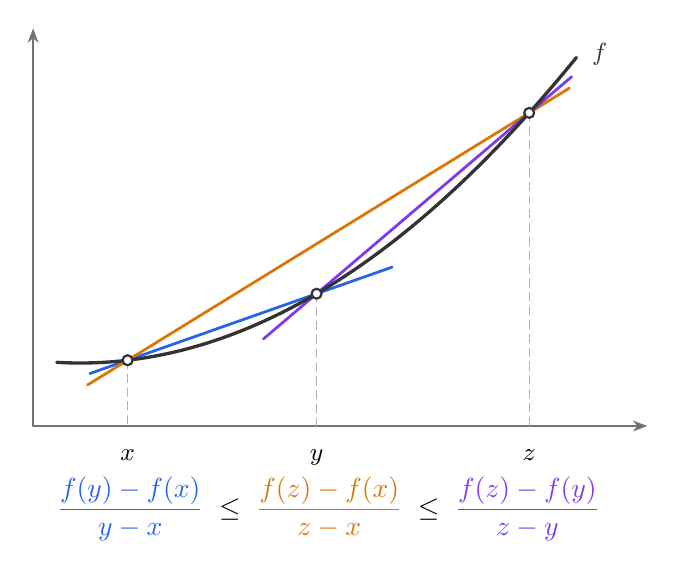
\begin{tikzpicture}[
  x=1.5cm, y=1cm,
  >=Stealth,
  line cap=round,
  line join=round,
  font=\small
]
  \definecolor{secantXY}{HTML}{2563EB}
  \definecolor{secantXZ}{HTML}{D97706}
  \definecolor{secantYZ}{HTML}{7C3AED}

  \coordinate (X) at (0.8,0.8352);
  \coordinate (Y) at (2.4,1.68);
  \coordinate (Z) at (4.2,3.9768);

  % 座標軸
  \draw[->,black!55,line width=0.5pt]
    (0,0) -- (5.2,0);
  \draw[->,black!55,line width=0.5pt]
    (0,0) -- (0,5.05);

  % 横軸への補助線
  \draw[black!30,densely dashed]
    (X) -- (0.8,0) node[below=5pt,text=black] {$x$};
  \draw[black!30,densely dashed]
    (Y) -- (2.4,0) node[below=5pt,text=black] {$y$};
  \draw[black!30,densely dashed]
    (Z) -- (4.2,0) node[below=5pt,text=black] {$z$};

  % 三つの割線
  \draw[secantXY,line width=1pt]
    ($(X)!-0.2!(Y)$) -- ($(X)!1.4!(Y)$);
  \draw[secantXZ,line width=1pt]
    ($(X)!-0.1!(Z)$) -- ($(X)!1.1!(Z)$);
  \draw[secantYZ,line width=1pt]
    ($(Y)!-0.25!(Z)$) -- ($(Y)!1.2!(Z)$);

  % 凸関数のグラフ
  \draw[black!80,line width=1.2pt,
        domain=0.2:4.6,samples=120]
    plot (\x,{0.22*(\x-0.4)^2+0.8});
  \node[right,text=black!80] at (4.65,4.72) {$f$};

  % グラフ上の三点
  \foreach \p in {X,Y,Z}{
    \filldraw[fill=white,draw=black!80,line width=0.8pt]
      (\p) circle[radius=1.8pt];
  }

  % 割線の色と傾きの対応
  \node[font=\normalsize] at (2.5,-1.05) {$\displaystyle
    \textcolor{secantXY}{\frac{f(y)-f(x)}{y-x}}
    \;\leq\;
    \textcolor{secantXZ}{\frac{f(z)-f(x)}{z-x}}
    \;\leq\;
    \textcolor{secantYZ}{\frac{f(z)-f(y)}{z-y}}
  $};
\end{tikzpicture}
\end{center}
\item
$f$はLipschitz連続である.

\item
任意の$a_0 \in I$に対して,
ある$a \in \R$が存在し,
任意の$x \in I$に対して,
\[
f(x) \geq f(a_0)+a(x-a_0)
\]

\item
（Jensenの不等式）
$(X,\mathcal{B},\mu)$を$\mu(X)=1$を満たす測度空間とし,
$g \colon X \to I$を可積分な可測関数とする.
このとき,
\[
f\left(\int_X g\,d\mu\right)
\leq
\int_X (f \circ g)\,d\mu
\]

\end{enumerate}
\end{lem}
\end{tcolorbox}

\begin{proof}
(1).
\(
y
=
\frac{z-y}{z-x}\,x
+
\frac{y-x}{z-x}\,z
\)
であるから, $f$の凸性より,
\begin{equation}
\label{eq-convex-1}
f(y)
\leq
\frac{z-y}{z-x}f(x)
+
\frac{y-x}{z-x}f(z)
\end{equation}
が成り立つ.
よって,
\[
\begin{aligned}
f(y)-f(x)
&\underalign{\eqref{eq-convex-1}}{\leq}
\frac{x-y}{z-x}f(x)
+
\frac{y-x}{z-x}f(z)
=
\frac{y-x}{z-x}\bigl(f(z)-f(x)\bigr).
\end{aligned}
\]
\[
\begin{aligned}
f(y)-f(z)
&\underalign{\eqref{eq-convex-1}}{\leq}
\frac{z-y}{z-x}f(x)
+
\frac{y-z}{z-x}f(z)
=
\frac{z-y}{z-x}\bigl(f(x)-f(z)\bigr).
\end{aligned}
\]

(2) 任意の$x_0 \in I$をとる.
\(
a<b<x_0<c<d
\)
を満たす$a,b,c,d \in I$をとる.
任意の$x,y \in [b,c]$で$x<y$を満たすものに対して,
(1)より,
\[
\frac{f(b)-f(a)}{b-a}
\leq
\frac{f(y)-f(x)}{y-x}
\leq
\frac{f(d)-f(c)}{d-c}
\]
が成り立つ.
そこで,
\[
L:=
\max\left\{
\left|\frac{f(b)-f(a)}{b-a}\right|,
\left|\frac{f(d)-f(c)}{d-c}\right|
\right\}
\]
とおくと,
\[
|f(y)-f(x)| \leq L|y-x|
\]
となる.
よって, $f$は$x_0$の近傍でLipschitz連続である.

(3) 任意の$x_0 \in I$をとる.
(1)より, 任意の$x,y \in I$で
$x<x_0<y$を満たすものに対して,
\[
\frac{f(x_0)-f(x)}{x_0-x}
\leq
\frac{f(y)-f(x_0)}{y-x_0}
\]
が成り立つ.
そこで,
\[
a_-:=
\sup_{x<x_0}
\frac{f(x_0)-f(x)}{x_0-x},
\qquad
a_+:=
\inf_{y>x_0}
\frac{f(y)-f(x_0)}{y-x_0}
\]
とおくと,
\(
a_- \leq a_+
\)
となる.
よって,
\(
a_- \leq a \leq a_+
\)
を満たす$a$をとれば, これが求めるものである.


(4) $I=(\alpha,\beta)$,
$-\infty \leq \alpha<\beta \leq \infty$とする.
\(
m:=\int_X g\,d\mu
\)
とおく.
$\alpha \in \R$のとき,
\[
m-\alpha
=
\int_X (g-\alpha)\,d\mu
>0
\]
であるから, $\alpha<m$となる.
同様に, $\beta \in \R$のとき, $m<\beta$となる.
したがって,
\[
m \in (\alpha,\beta)=I.
\]

(3)より, ある$a \in \R$が存在して,
任意の$t \in I$に対して,
\[
f(t) \geq f(m)+a(t-m)
\]
が成り立つ.
$t=g(x)$とすると, 任意の$x \in X$に対して,
\[
f(g(x))
\geq
f(m)+a\bigl(g(x)-m\bigr)
\]
となる.
両辺を積分して,
\[
\int_X (f \circ g)\,d\mu
\geq
\int_X \bigl(f(m)+a(g-m)\bigr)\,d\mu.
\]

\end{proof}


\end{document}